\documentclass{article}
\usepackage{amsmath,amsthm,amssymb}
\usepackage{mathtext}
\usepackage[T1,T2A]{fontenc}
\usepackage[utf8]{inputenc}
\usepackage[english,bulgarian,ukranian,russian]{babel}
\usepackage[utf8]{inputenc}
\usepackage{tikz}
\usepackage{pdfpages}
\usepackage{graphicx}
\usepackage{float}
\usepackage[T2A]{fontenc}
\usepackage[utf8]{inputenc}
\usepackage[russian,english]{babel}
\usepackage[options]{natbib}



\title{Определение местоположения по сигналу акселерометра}


\author{\bf \em Zaynulina E. T., Kiseleva E. A., Protasov V. P., Fateev D. A.,\\
 \bf \em Bozhedomov N., Tolkanev A. A., Nochevkin V., Ryabov A. }

\date{October 2018}

\begin{document}

\maketitle

\section{Краткий обзор}
Данная статья посвящена использованию методов машинного обучения в задаче определения
местоположения по показаниям носимых человеком сенсоров. Задача является актуальной и имеет такое применение, как,
например, автоматическое включение/выключение энергозатратных сервисов при различном
положении мобильного устройства. Поставленная задача решается по сигналам датчика телефона – акселерометра. Основной цель работы – это способ
выбора и предобработки признаков, позволяющий уменьшить влияние шума на результат
классификации и анализировать активность в независимости от пространственной
ориентации мобильного устройства. Результаты, полученные в ходе вычислительного эксперимента,
подтверждают применимость предложенного подхода.

\bigskip

Современные смартфоны обладают большим числом сенсоров и высокой вычислительной способностью. Так как в настоящее время почти каждый человек им обладает, то методы определения местоположения человека с использованием смартфонов получили наибольшее внимание со стороны исследователей. Среди этих методов - методы, основанные на беспроводных сигналах (WiFi, Bluetooth, UWB)\cite{journals/puc/VeraOA11}\cite{journals/puc/KimJP13}, датчиках обзора (лазерный сканер, монокулярная и бинокулярная камера)\cite{journals/puc/BrunsB09}, инерционных датчиках (акселерометр, гироскоп, магнитометр)\cite{journals/puc/ParkSC13}\cite{journals/puc/HardeggerRT15}\cite{journals/sensors/WangLYJG18}\cite{6987239}. Многие из предложенных методов локализации человека представляют собой комбинацию выше перечисленных для увеличения точности позиционирования\cite{journals/ejasp/EvennouM06}\cite{6834746}\cite{7021969}. Методы, основанные на беспроводных сигналах и датчиках обзора, помимо наличия смартфона требуют также введения дополнительного оборудования либо наличия дополнительных знаний, например карты помещения или базы данных силы сигнала (RSSI) WiFi точки в зависимости от координаты (WiFi fingerprint). Однако не всегда возможно предоставить карту помещения, например, в силу конфиденциальности; вспомогательное оборудование, в свою очередь, требует технического обслуживания и больших затрат. Что касается WiFi позиционирования, то при наличии существующей базы данных WiFi fingerprint при некотором изменении среды, позиционирование будет неточным, поэтому база данных нуждается в постоянном обновлении\cite{journals/sensors/Torres-Sospedra17a}.

Чтобы избежать данных проблем, предлагается метод, основанный на инерционных датчиках. В качестве базового алгоритма рассматривается pedestrian dead reckoning (PDR)~\cite{7743695}. По сравнению с методами, основанными на беспроводных сигналах и датчиках обзора, PDR рассчитывает относительно точное местоположение человека быстрее и потребляя меньше вычислительной мощности. Для фильтрации шума в данных используется фильтр Калмана~\cite{journals/corr/abs-1712-09004}. Особенность данной работы состоит в том, чтобы восстанавливать траекторию не от точки к точке, а всю целиком. Для работы с полученным многомерным пространством предлагается использовать метод PLS\cite{10.1007/11752790_2}.


{\bf Новизна:} задача исследования ставится в терминах projection to the latent space (It is pretty much used that way in machine learning — you observe some data which is in the space that you can observe, and you want to map it to a latent space where similar data points are closer together.)



{\bf Ключевые слова:} обработка сигналов; сенсоры; акселерометр; анализ данных; машинное обучение, инерциальные методы, позиционные методы
\section{Введение}

Задача определения местоположения произвольного телефона для любого пользователя
является сложной по следующим причинам: манера движения, в частности походка,
у людей сильно различается; характеристики одежды, карманов и сумок варьируются
в широких пределах, ориентация телефона в пространстве может быть произвольной.
Датчики мобильных устройств имеют значительный разброс параметров

\section{Постановка задачи}

При решении задачи используются данные, полученные с помощью инерционных датчиков. Эти данные представляются в виде многомерных временных рядов $s(t) \in \mathbb{R}^N$. Каждому временному ряду ставится в соответсвие вектор признаков. Эти вектора образуют матрицу признаков $X \in \mathbb{R}^{N \times T}.$ По данной матрице предсказывается матрица траекторий пешехода вида $Y \in \mathbb{R}^{N \times T}$, а строками данной матрицы являются временные ряды $y(t)$, демонстрирующие изменение положения по широте и долготе в течение времени. Модель имеет вид:  \[f: X \to Y\]

Используемые в задаче данные, были собраны с разных расположений датчиков: рюкзак, нога, рука, туловище. Поэтому задача разбивается на две: определение класса расположения датчика $(P)$ и предсказание самой траектории перемещения на основе решения первой задачи:
\[f_1: X \to P = \{0, 1, 2, 3\}\]
\[f_2: X,P \to Y\]

Для решения задач используемся метод опорных векторов(SVM) для случая линейной неразделимости классов, который минимизирует следующий функционал $S(w|f,X,Y)$ и введём штраф за суммарную ошибку:

\[\min_{w, w_0}S(w, w_0) = \frac{1}{2}\|w\|^2+C\sum_{i=1}\xi_i\] 

где $C$ - параметр настройки метода,  $\xi_i$ - набор дополнительных переменных характеризующих величину ошибки на объектах $x_i$, вектор $w$ - перпендикуляр к разделяющей гиперплоскости.

При условиях:
\[y_i(w^Tx_i+w_0)\geq 1-\xi_i\]
\[\xi_i \geq 0~\forall i\]

Для оценки качества модели используется критерий суммы квадратов отклонений предсказанных координат от истинных, а также корреляция между предсказанной и истинной траекториями пешехода.

Формально постановку задачи следует записать следующим образом:
\[w^* = \arg\min_{w}S(w|f, X, Y).\]

\section{Базовый алгоритм}
В ходе получения матрицы признаков $X$ в данных подавляются шумы высокой частоты с помощью применения Гауссового сглаживания с разными параметрами для 6-ти каналов гиростабилизатора(IMU channels) и 2-ух скоростных каналов. Преобразуем сглаженные угловое и линейные ускорения в вектор признаков.

В качестве базового алгоритма используется каскадная регрессия состоящая из модели вида:
\begin{itemize}

\item подаются данные на вход SVM классификатора, который уже их разделяет на 4 класса: нога, сумка, рука, тело
\item далее полученные данные идут вход на 2 SVR-регрессора для каждого класса, которые обучаются на тренировочных данных, которые в итоге выдают скорости передвижения человека для каждого временного блока. Именно 2 SVR-регрессора для предсказания двумерной скорости в IMU-стабилизированной системе координат, игнорируя вертикальную составляющую.
\end{itemize}

Но полученные векторы скоростей содержат ошибки, которые связаны с неточностями инерционных датчиков: системой ротации. Поэтому делается предположение о низкочастотных смещениях в линейном ускорении. Этот подход не имеет явных физических обоснований, но позволяет обойти явное моделирование шумов / смещений и сводит задачу к задаче минимизации:

\[\min_{\{x^1_I, x^51_I,\dots\}}V_{bias}=
\min_{\{x^1_I, x^51_I,\dots\}}\sum_{f \in F_2}\|v_C^F-v_R^f\|+
\lambda\sum_{f \in F_1}\|x^f_I\|^2,\]
\[v_C^f = R_{SW}^f\sum_{f'=1}^f R_{WI}^{f'}(a_I^{f'}+x_I^{f'}),\]
где $f$ - единица блока выборки, $F$ - блок выборки, $v_C^F$ - скорректированное значение скорости, $v_R^f$ - предсказанное значение скорости, $I$ - система координат устройства, $W$ - глобальная система координат, $S$ - IMU-стабилизированная система координат, $R_{AB}$ - матрица перехода из системы координат $B$ в систему координат $A$.

\bigskip

Для каждого класса создается SVR-регрессор, предсказывающий угловые скорости пешехода в каждом временном блоке. 

На контрольной выборке для SVM-классификатора и каждого SVR-регрессора подбираются оптимальные значения гиперпараметров.

По полученным значениям скоростей восстанавливается траектория пешехода.

После получения из данных матрицы признаков $X$

Формально алгоритм описывается следующим образом: 


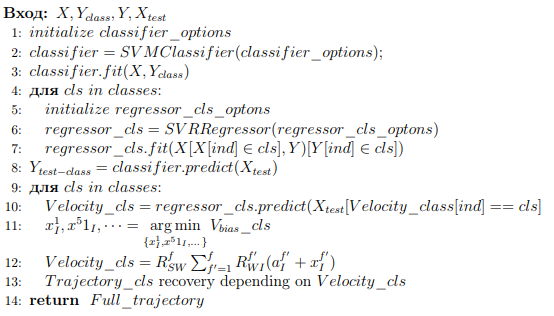
\includegraphics{new}

\section{Эксперимент}

Цель эксперимента: найти параметры модели для более точного предсказания исходной траектории.

В ходе эксперимента используются данные в статье, исследуемой алгоритм RIDI[14]. Данные были собраны с помощью инерционных датчиков смартфона с разным расположением: в руке, на ноге, в сумке и на поясе. Выборки содержат траектории с временным блоком в 100 минут и частотой сигнала 200 Гц.

В качестве объекта рассматривается положение в определенный момент времени $i$. Признаками объекта являются угловые скорости и линейные ускорения в стабилизированной системе координат датчиков в моменты времени $i-window\_size, \dots, i$, где $window\_size$ - размер окна (равен 200). Целевыми переменными являются метки классов, характеризующие то, в каком положении находился смартфон при получении определенных данных, а также скорости в данный момент времени $i$, которые вычисляются через координаты пешехода и прошедшее время. По полученным данным после уточнения скоростей с помощью оптимизации функции  $V_{bias}$ строится предсказанная траектория пешехода.

В ходе эксперимента исследовалась зависимость качества моделей на контрольной выборке в зависимости от параметров SVM-регрессоров.  Во всех моделях в качестве ядер были выбраны радиальные базисные функции, подбирались такие параметры как коэффициент штрафа $C$ и ядерный коэффициент $\gamma$. Качество измерялось с помощью кросс-валидации. Из результатов эксперимента следует, что для каждого расположения смартфона и каждого канала данных должны быть выбраны свои параметры модели.  Это подтверждает разумность классификации типа расположения смартфона перед непосредственным предсказанием траектории. 

Графики зависимости качества предсказания модели от параметров:

\begin{enumerate}
\item Выборка 1 состоит из 30742 объектов (8728 объектов класса рука, 6106 объектов класса нога, 7758 объектов класса тело, 8150 объектов класса сумка).
    
\item Выборка 2 состоит из 42731 объектов (13204 объектов класса рука, 8083 объектов класса нога, 11105 объектов класса тело, 10339 объектов класса сумка).
    
\item Выборка 3 состоит из 35892 объектов (9458 объектов класса рука, 7304 объектов класса нога, 13306 объектов класса тело, 5824 объектов класса сумка).
    
\end{enumerate}

    \begin{figure}[H]
    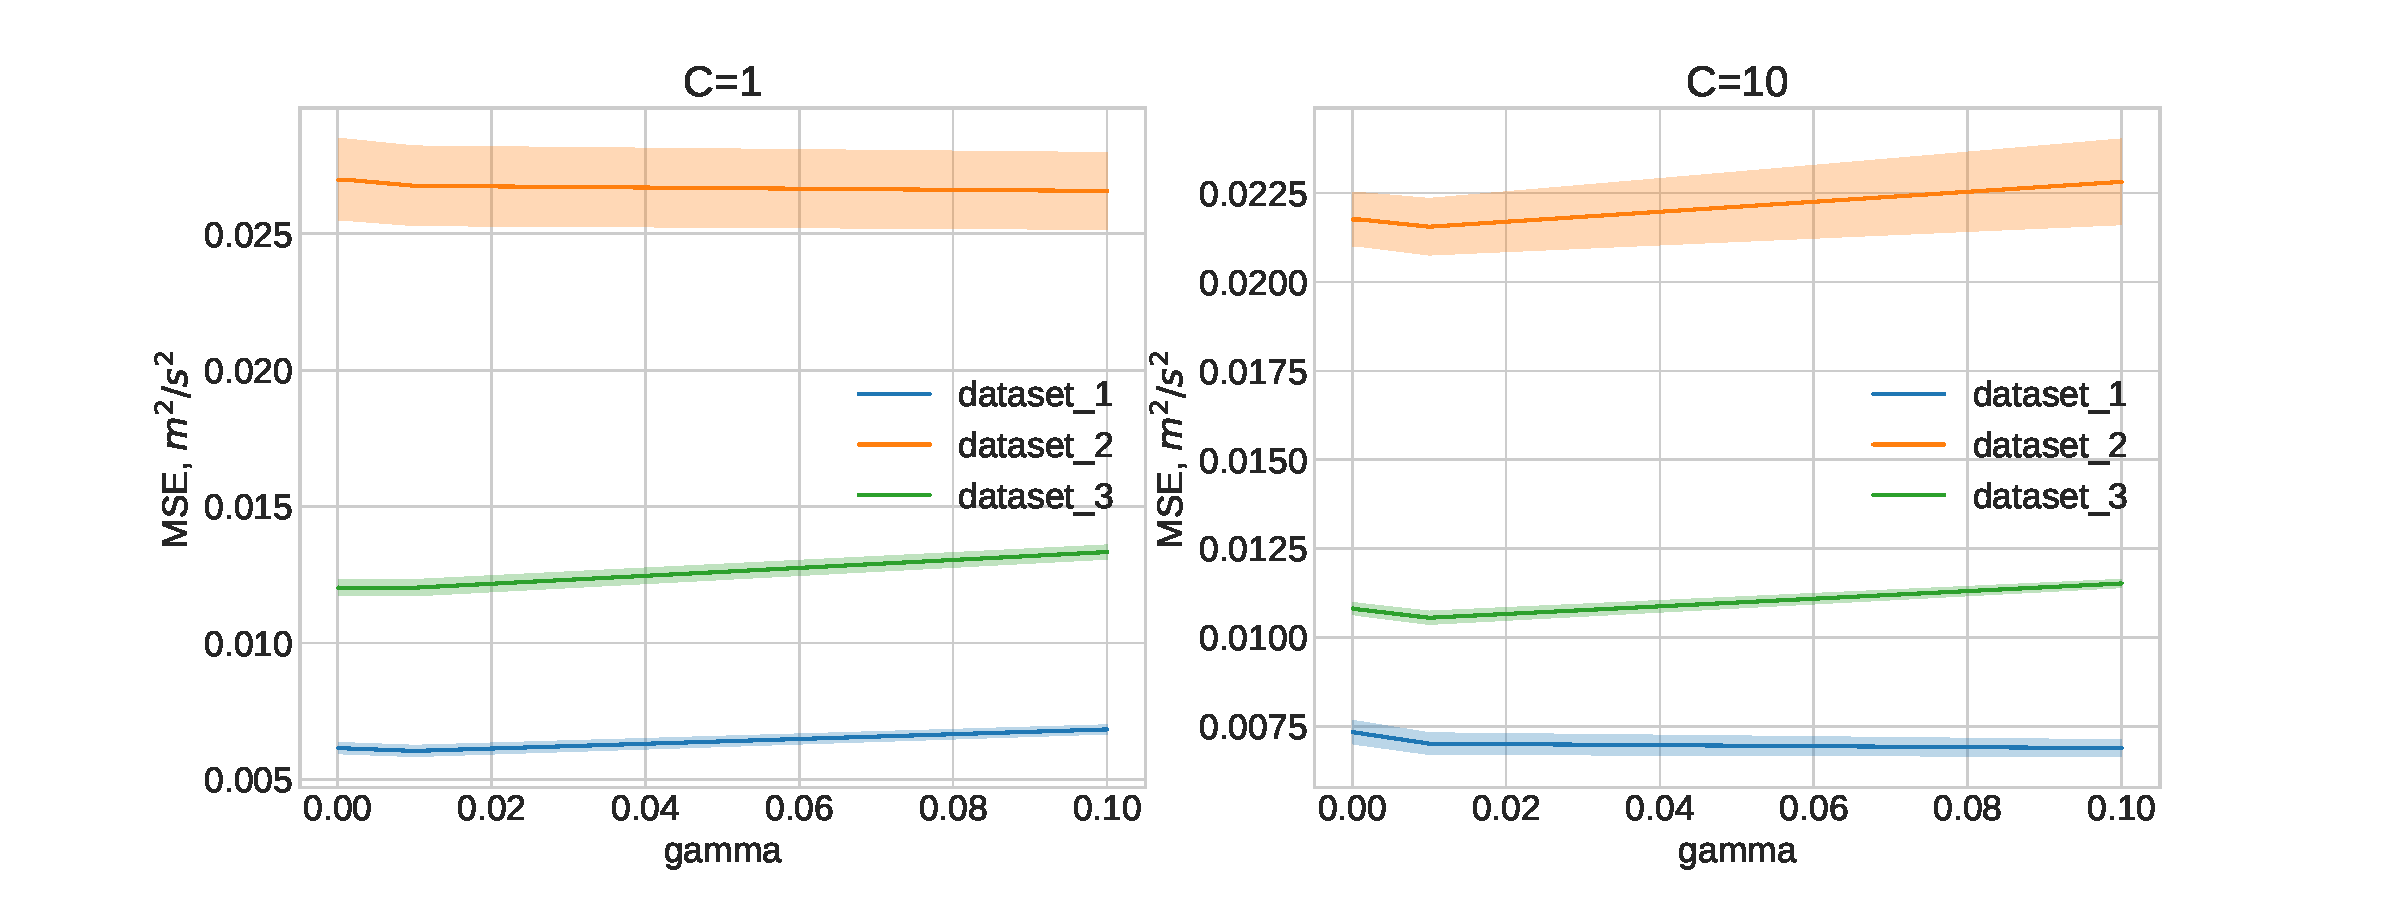
\includegraphics[scale=0.4]{charts/handheld_chn0_C=10.pdf}
    \caption{Рука, канал 0}
    \label{fig:image}
    \end{figure}
    
    \begin{figure}[H]
    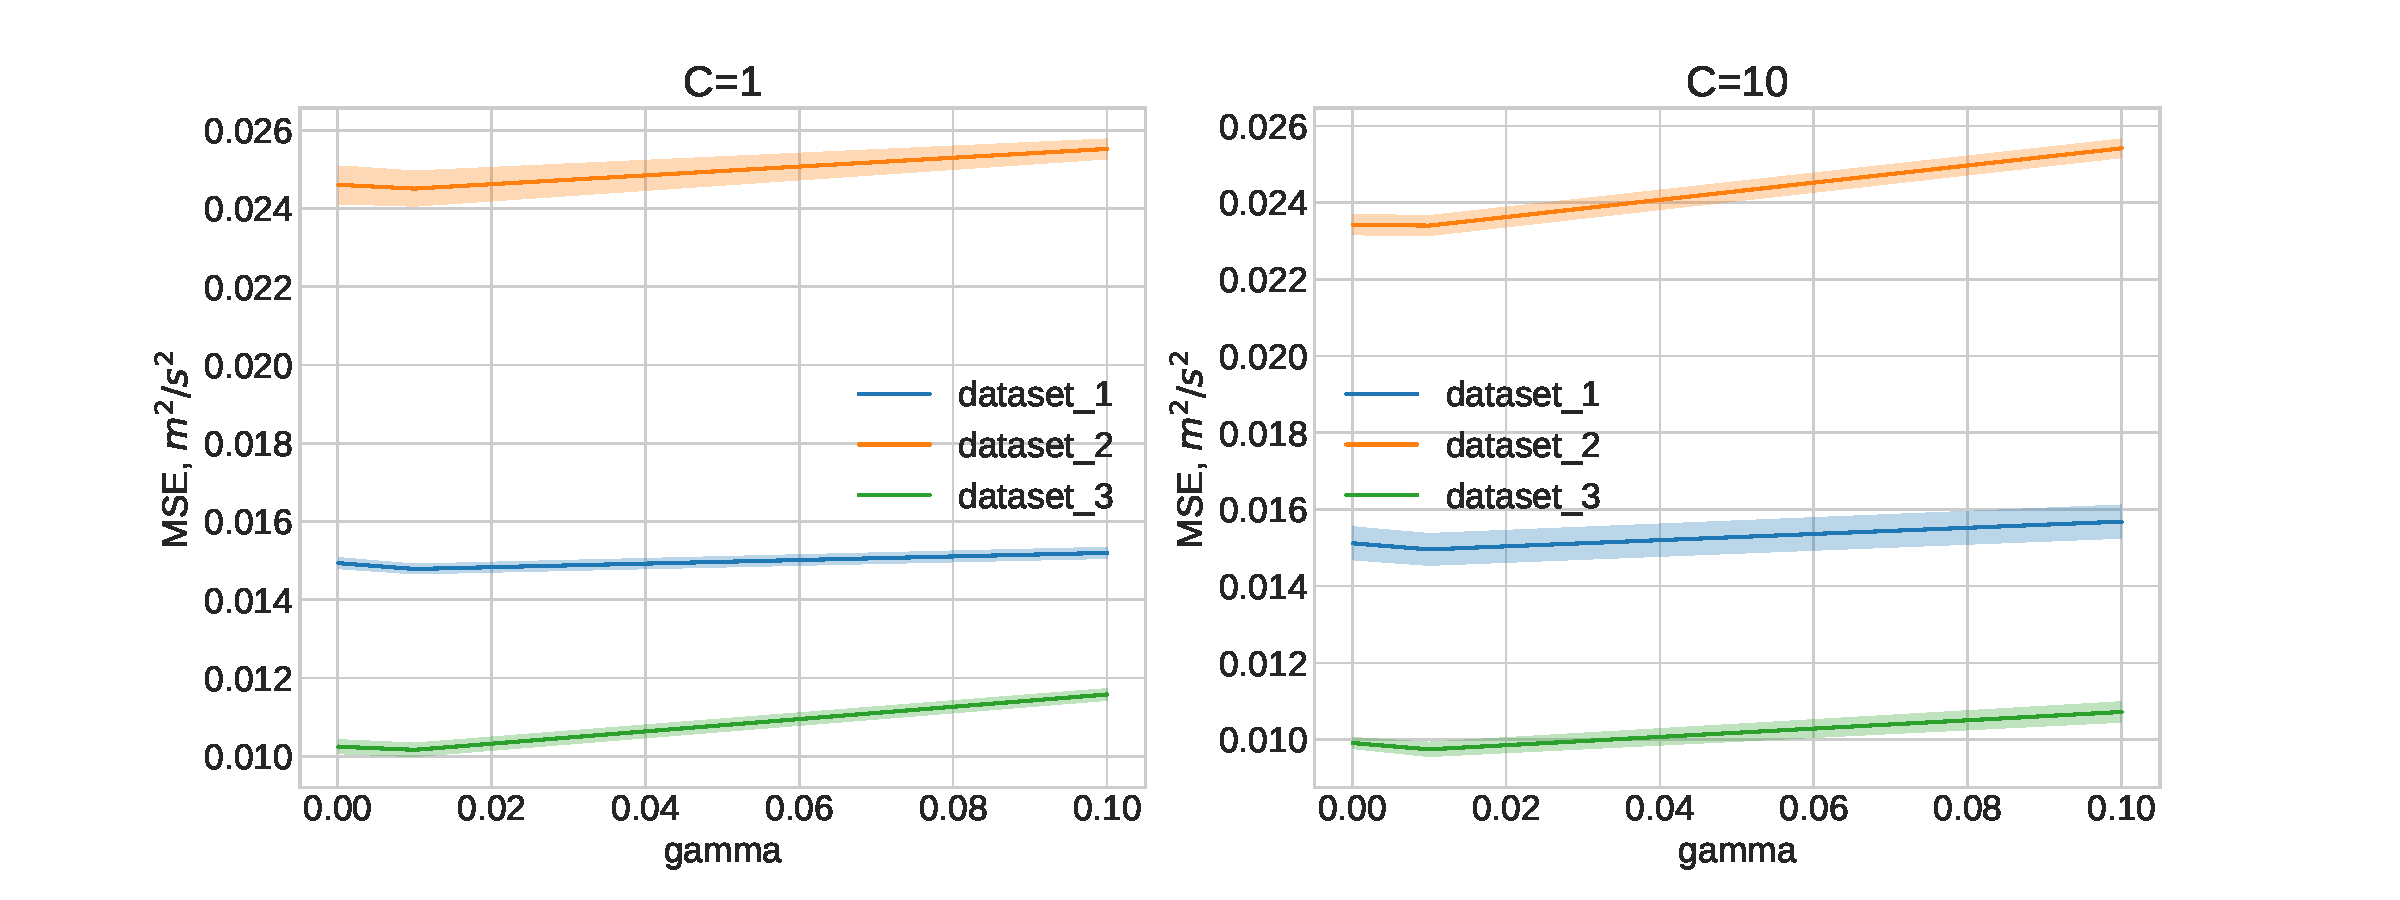
\includegraphics[scale=0.4]{charts/handheld_chn1_C=10.pdf}
    \caption{Рука, канал 1}
    \label{fig:image}
    \end{figure}
    
    \begin{figure}[H]
    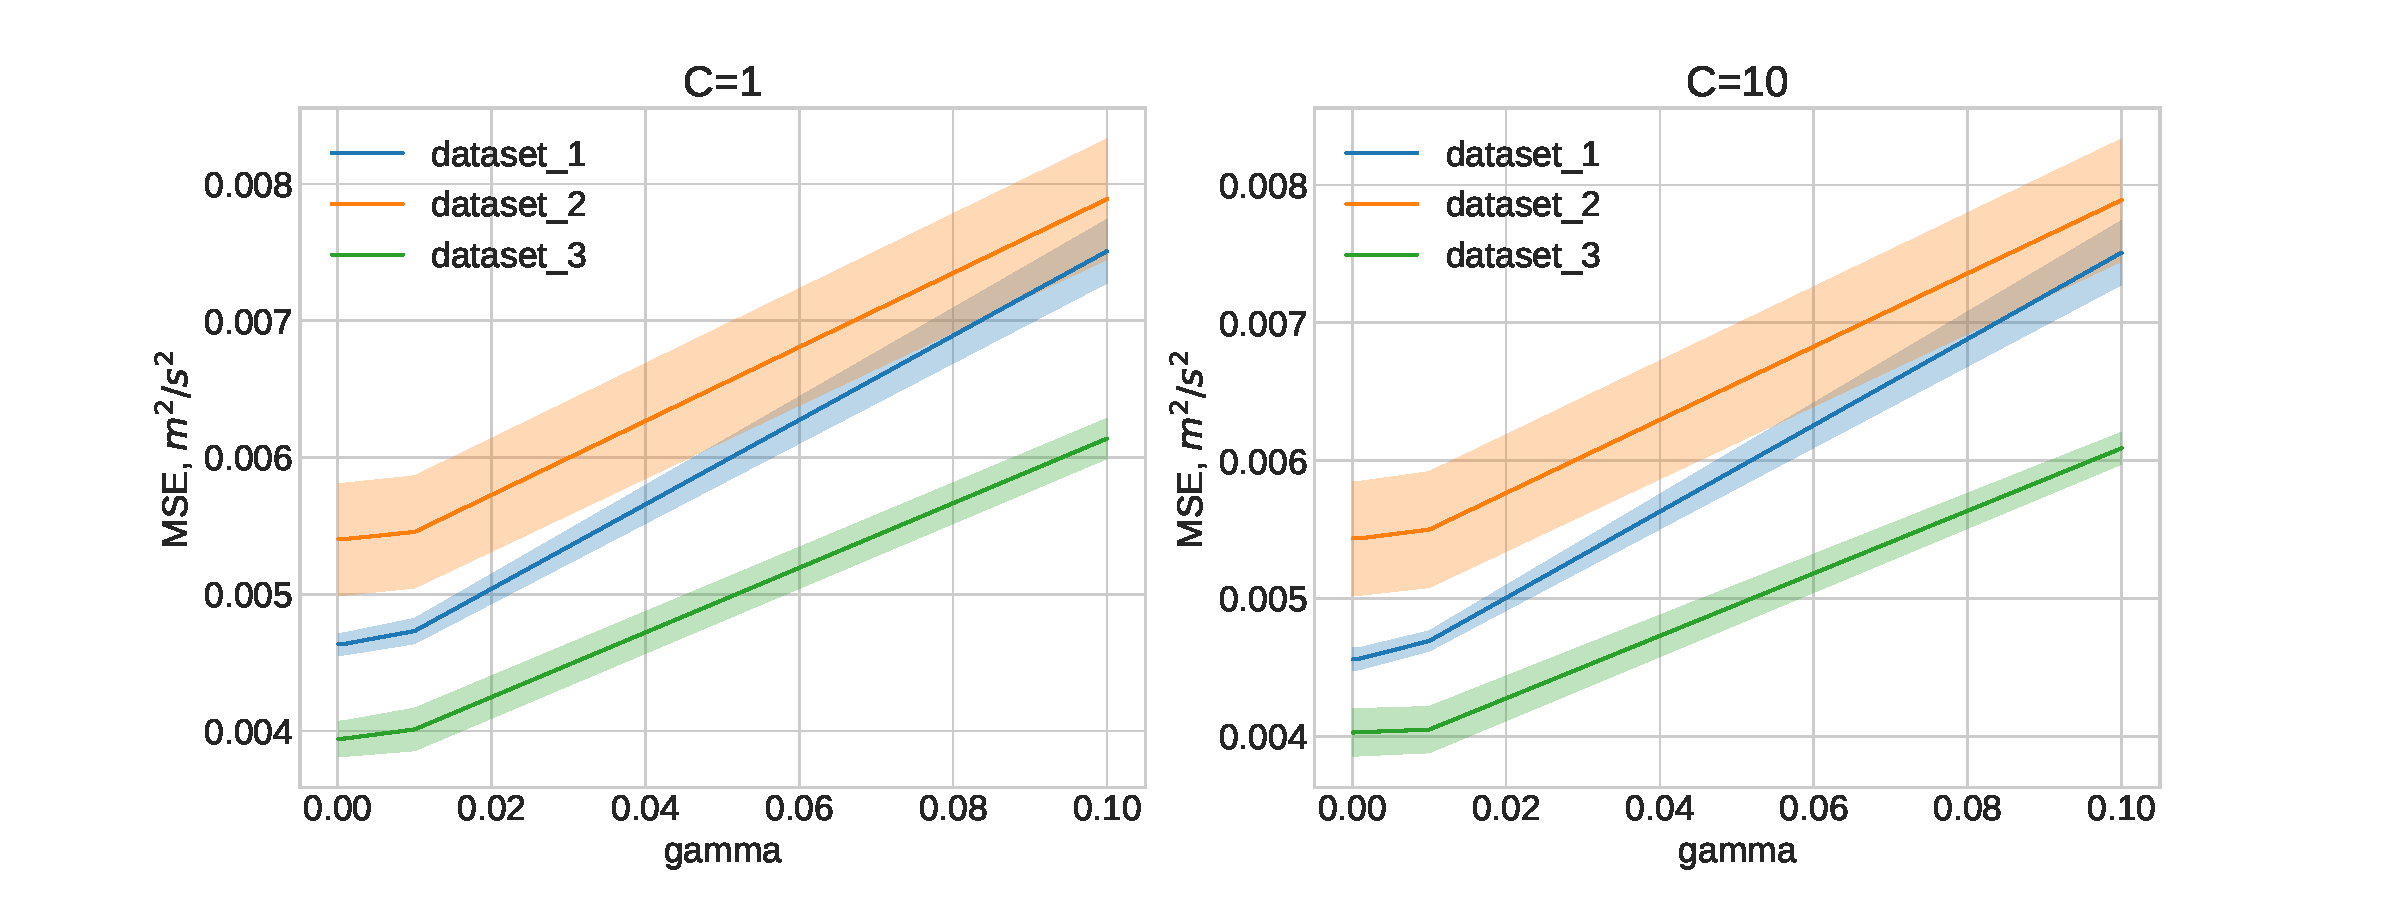
\includegraphics[scale=0.4]{charts/leg_chn0_C=10.pdf}
    \caption{Нога, канал 0}
    \label{fig:image}
    \end{figure}
    
    \begin{figure}[H]
    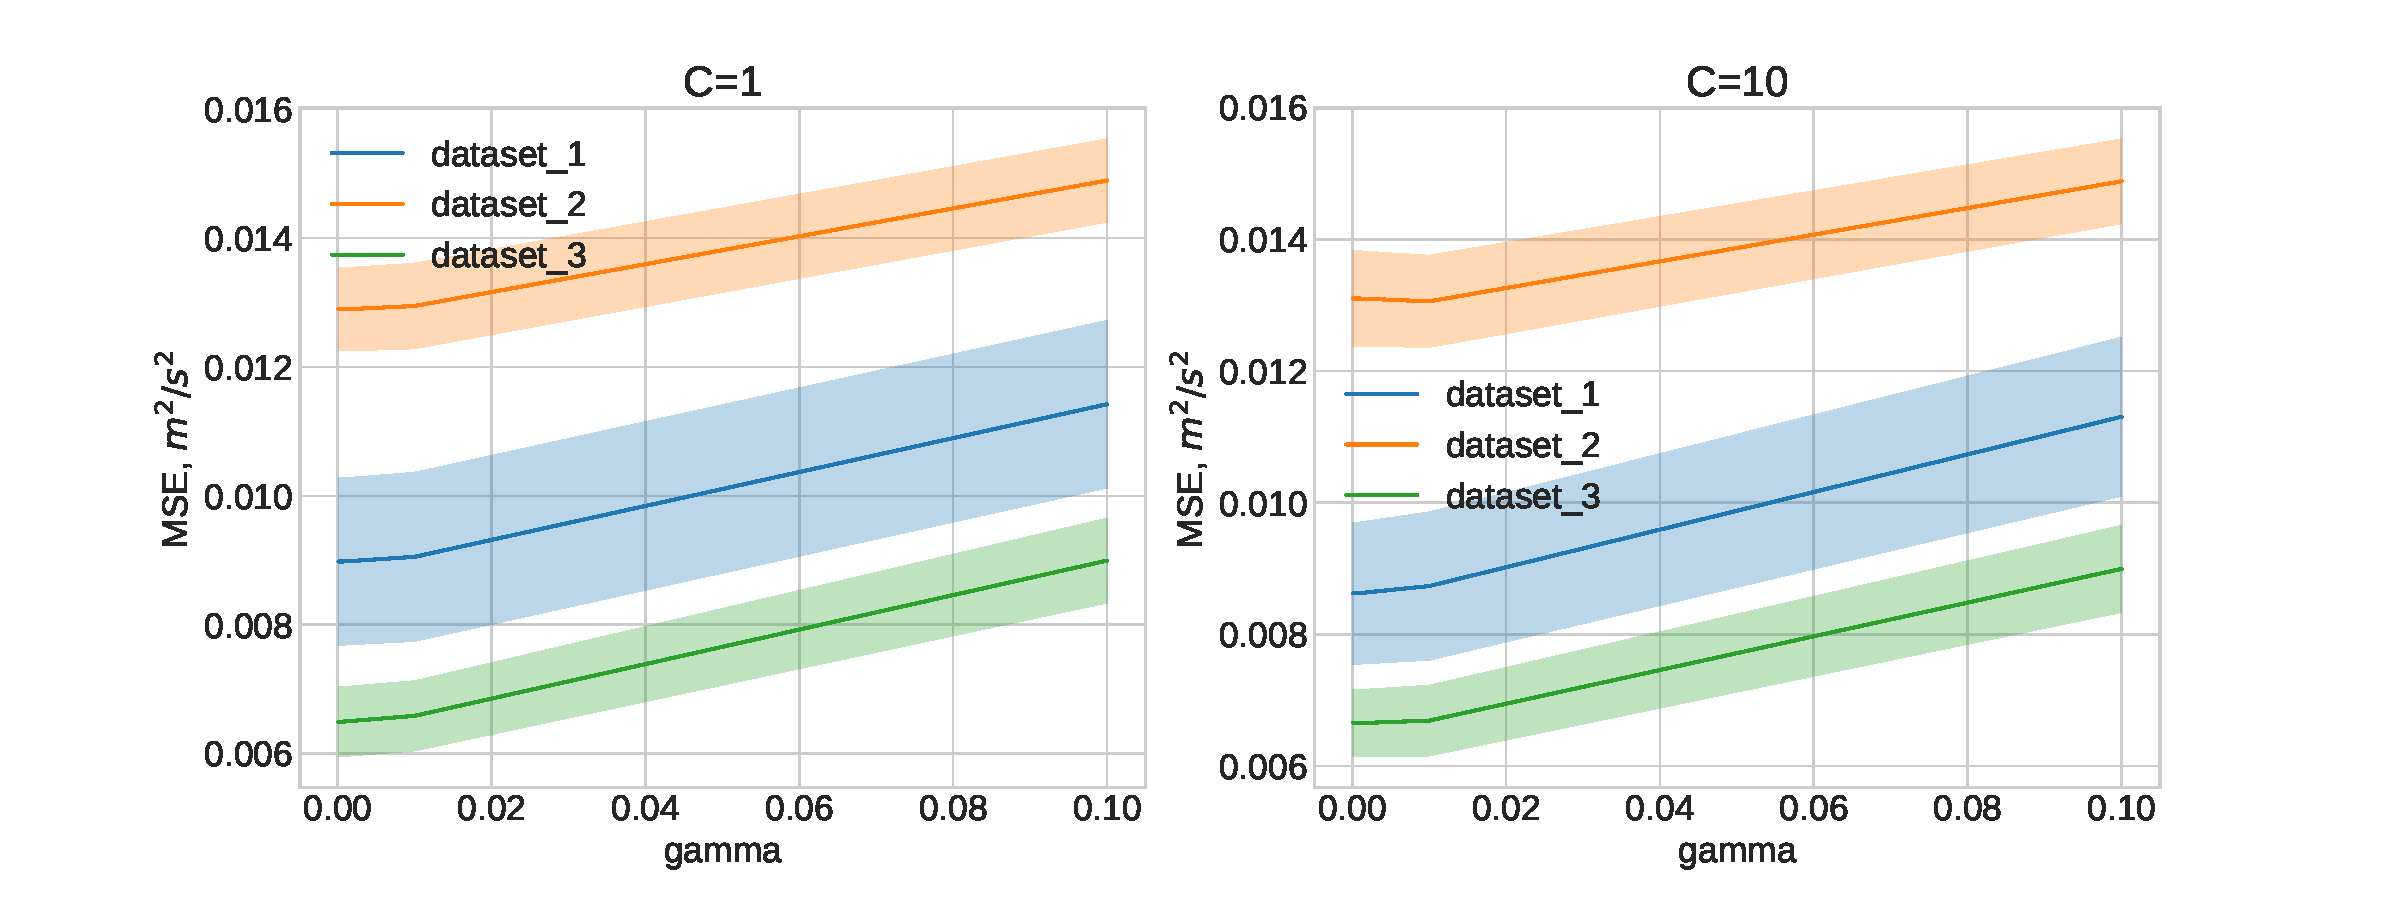
\includegraphics[scale=0.4]{charts/leg_chn1_C=10.pdf}
    \caption{Нога, канал 1}
    \label{fig:image}
    \end{figure}
    
    \begin{figure}[H]
    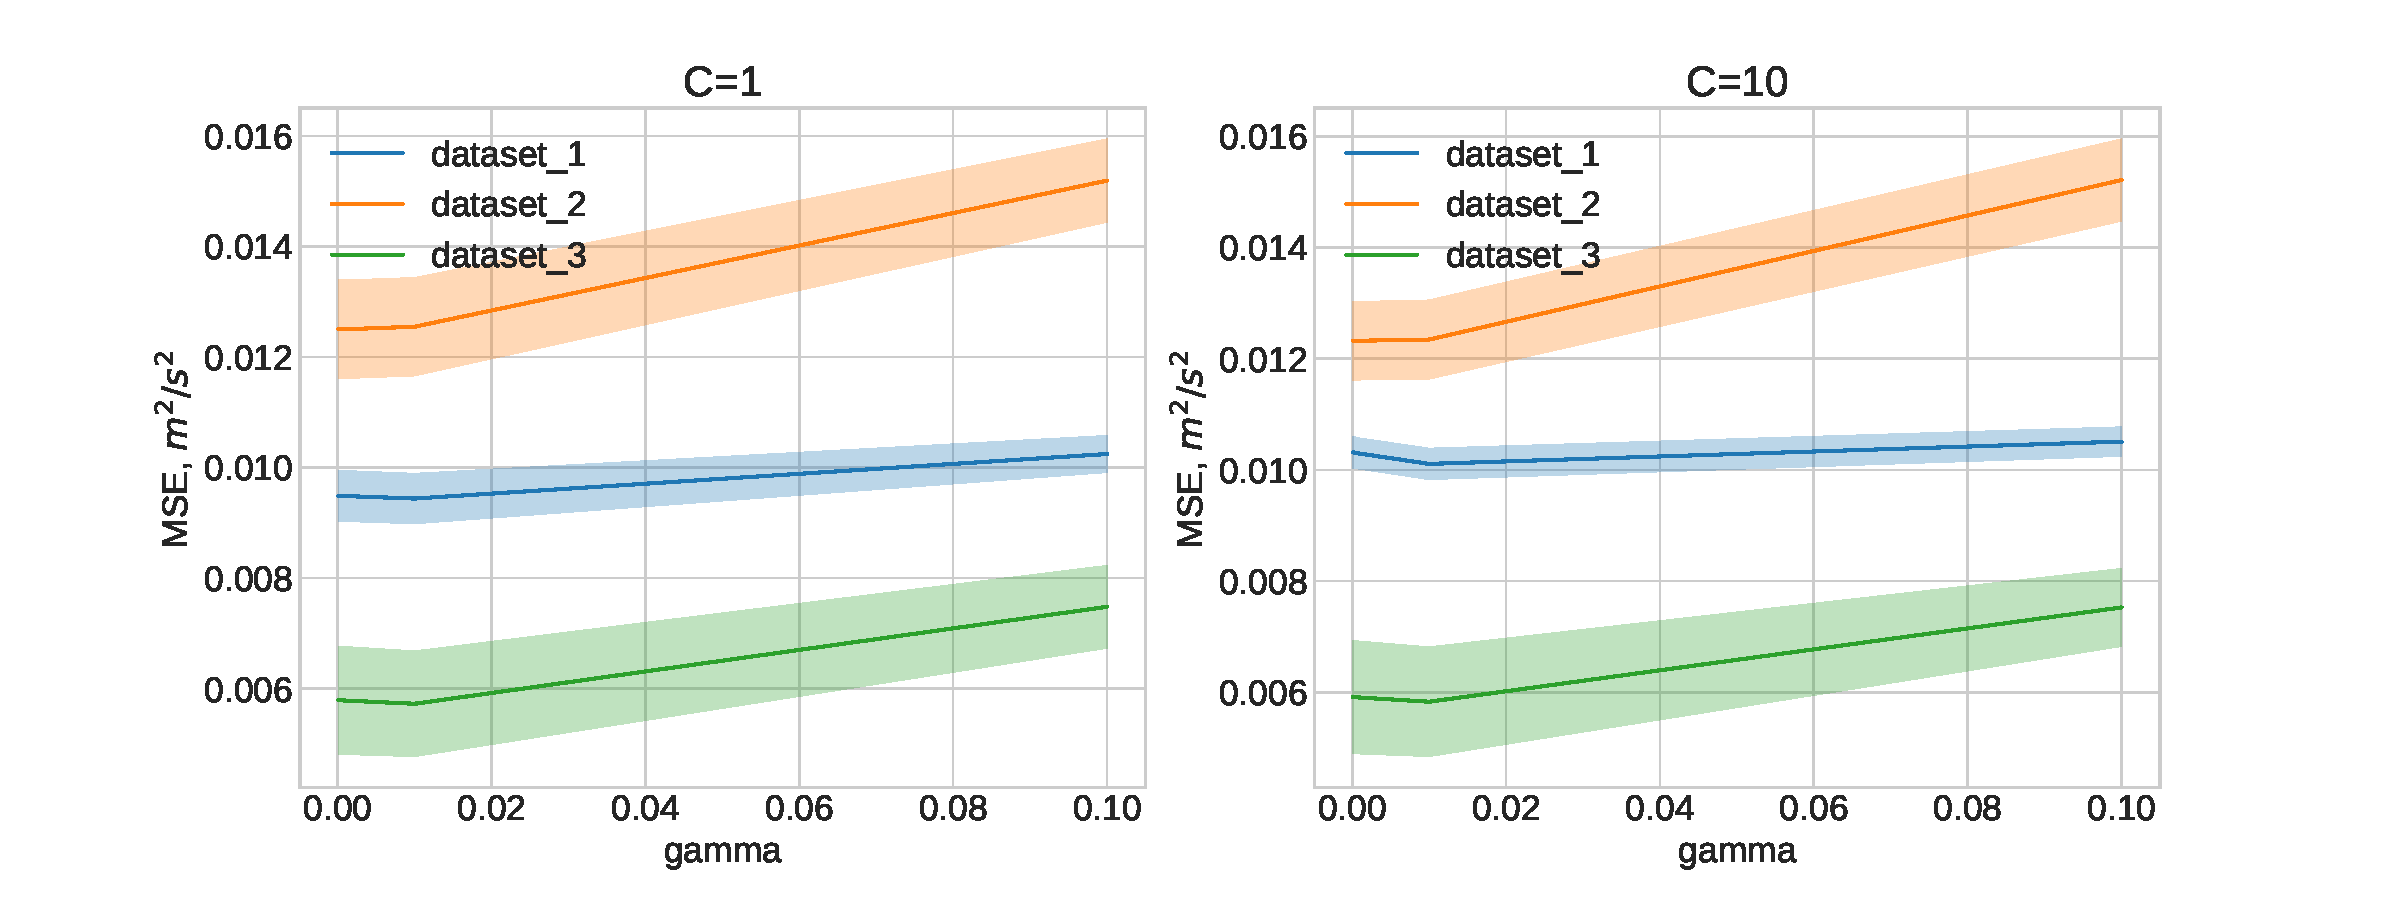
\includegraphics[scale=0.4]{charts/bag_chn0_C=10.pdf}
    \caption{Сумка, канал 0}
    \label{fig:image}
    \end{figure}
    
    \begin{figure}[H]
    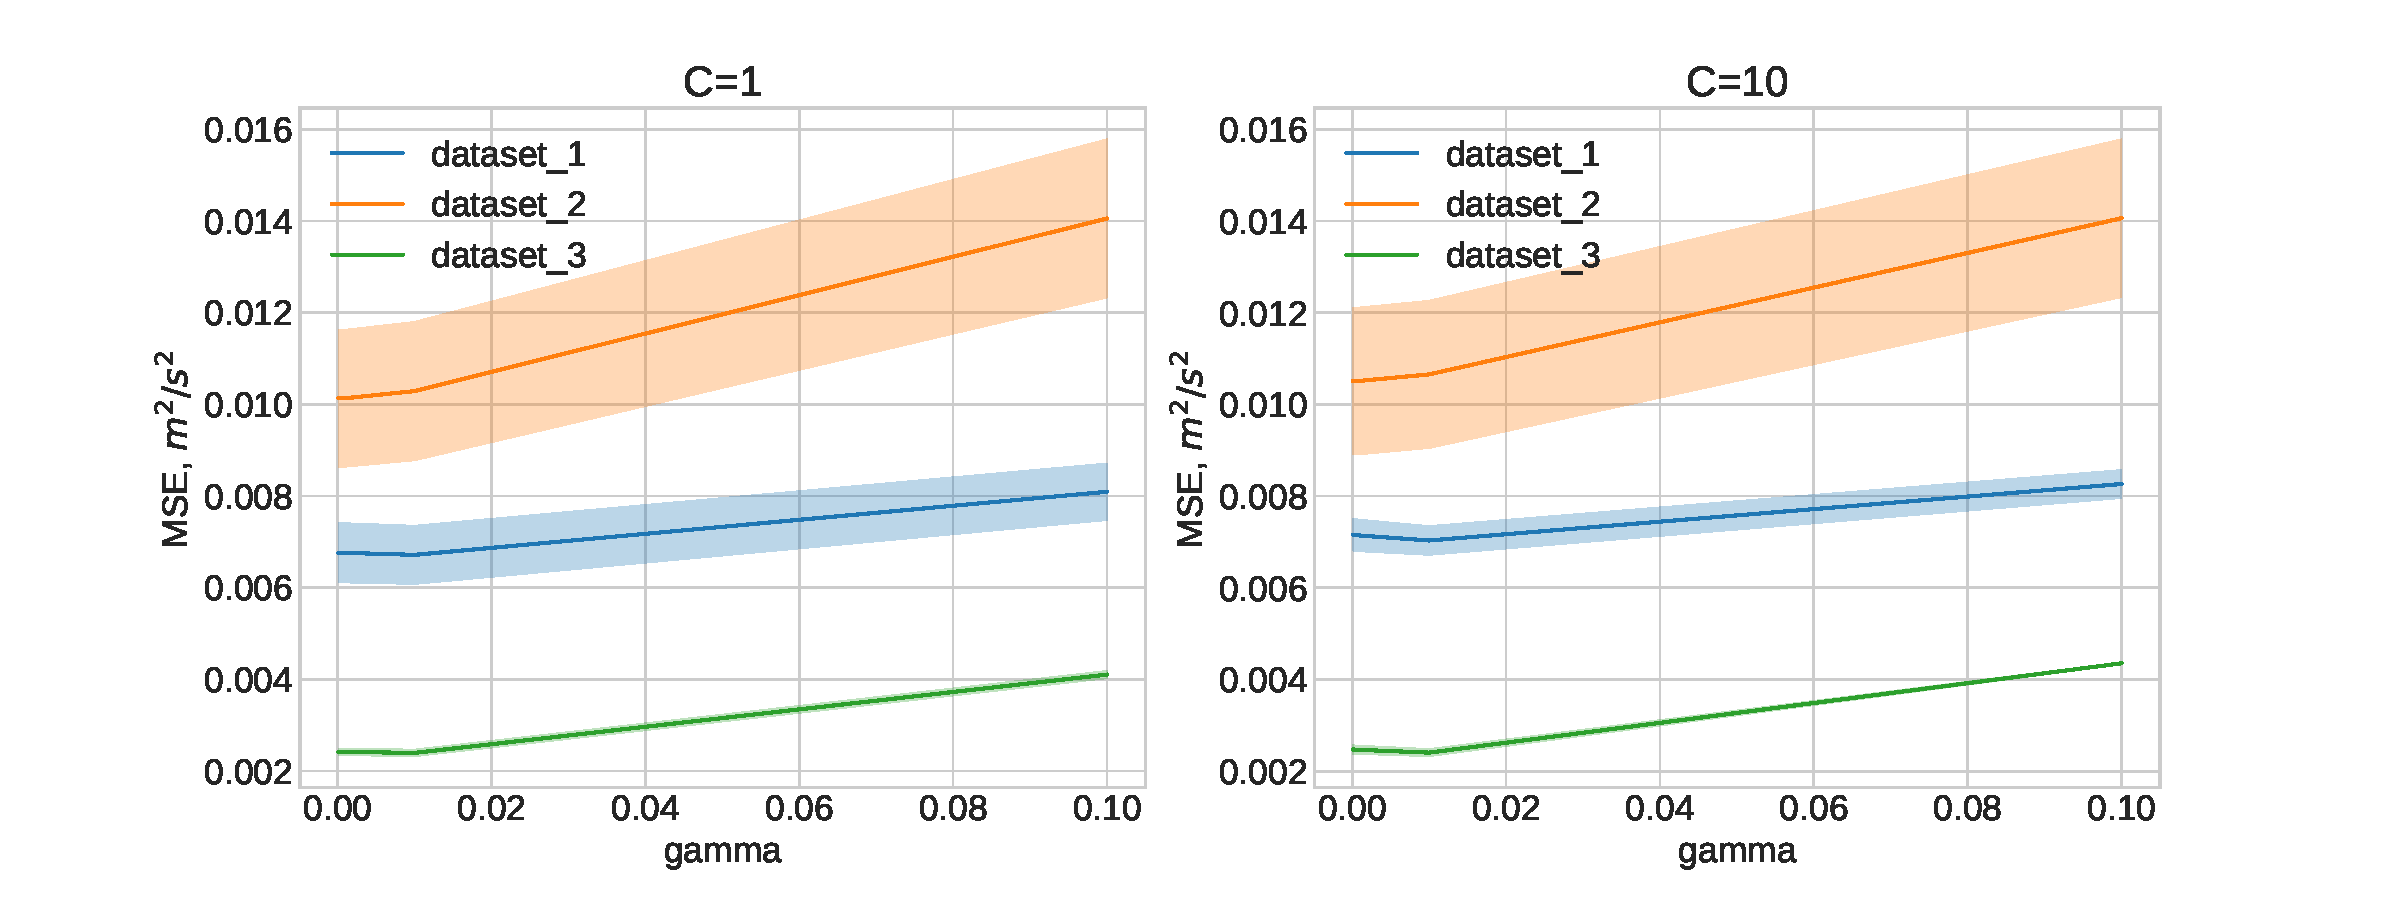
\includegraphics[scale=0.4]{charts/bag_chn1_C=10.pdf}
    \caption{Сумка, канал 1}
    \label{fig:image}
    \end{figure}
    
    \begin{figure}[H]
    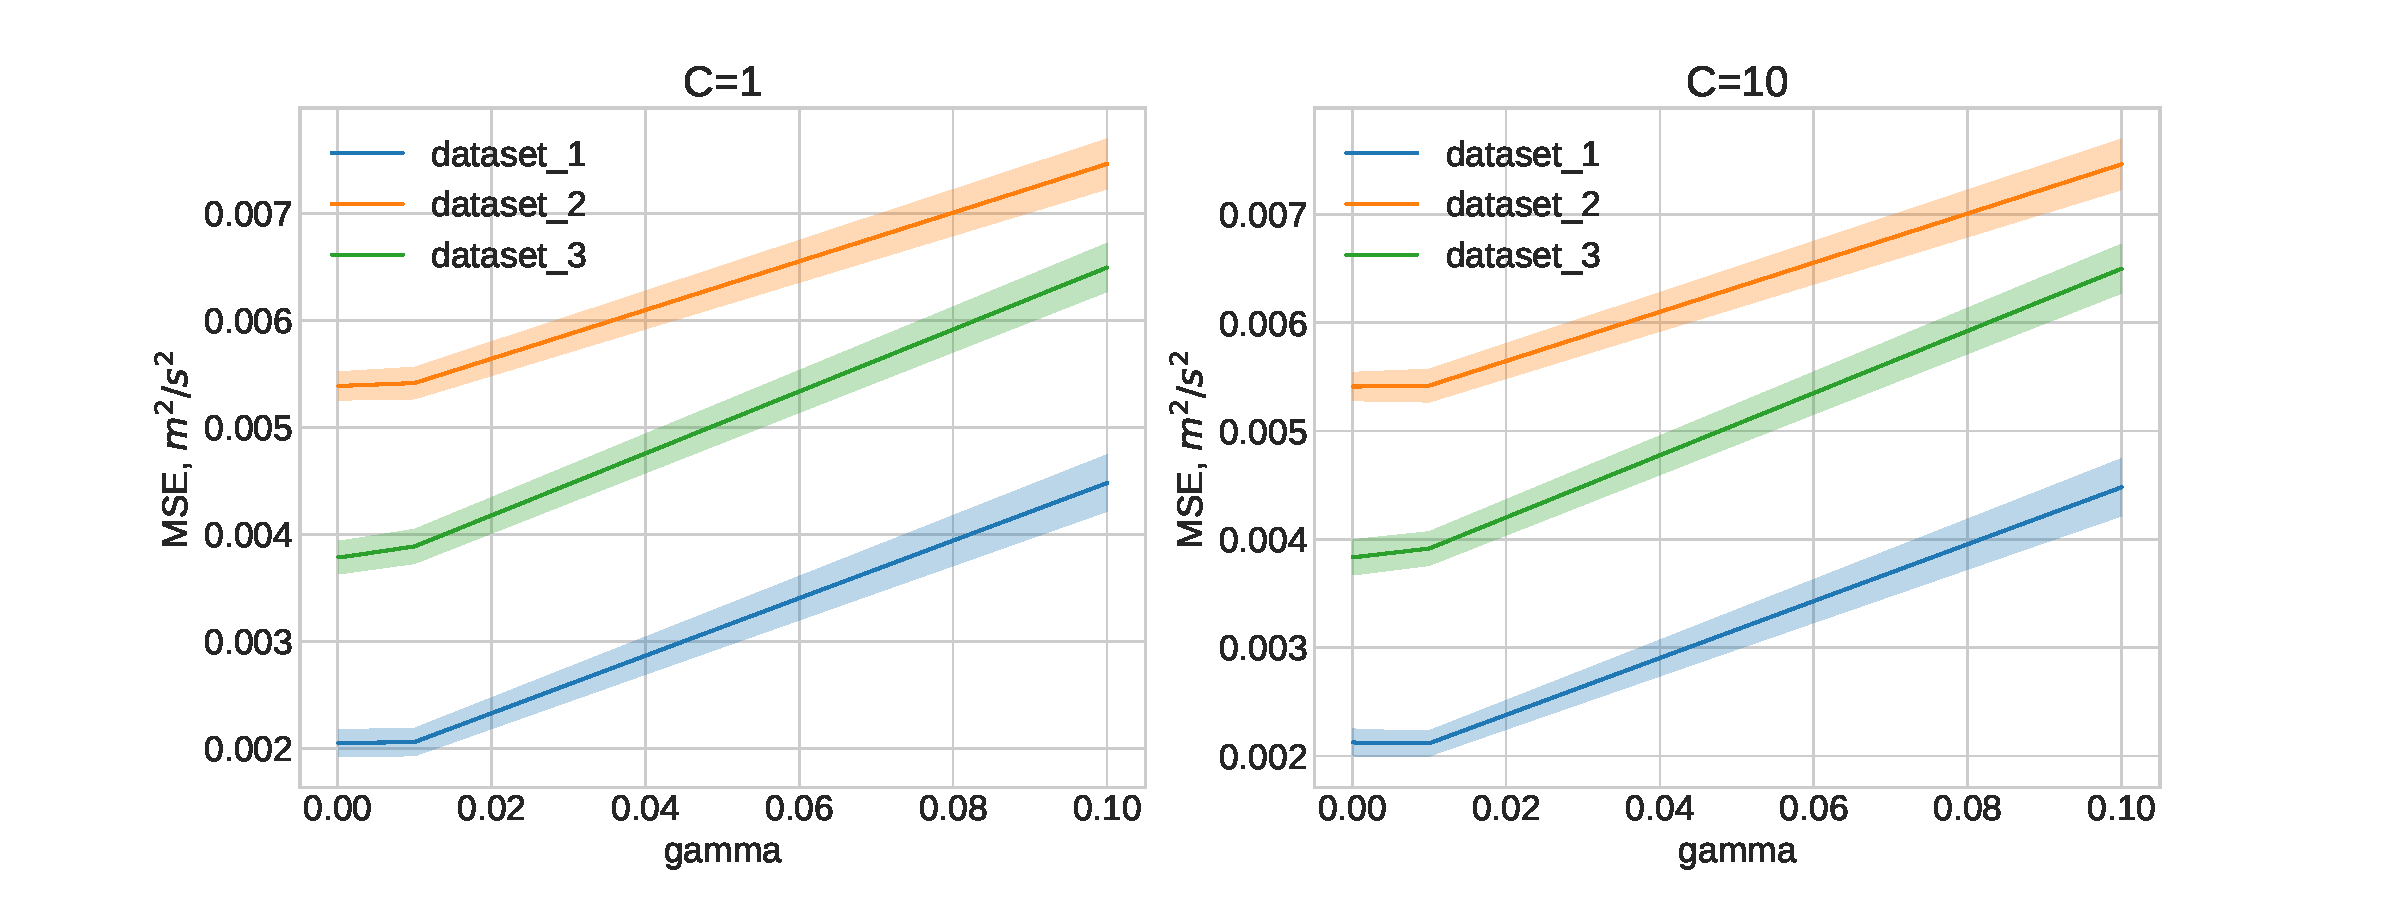
\includegraphics[scale=0.4]{charts/body_chn0_C=10.pdf}
    \caption{Тело, канал 0}
    \label{fig:image}
    \end{figure}
    
    \begin{figure}[H]
    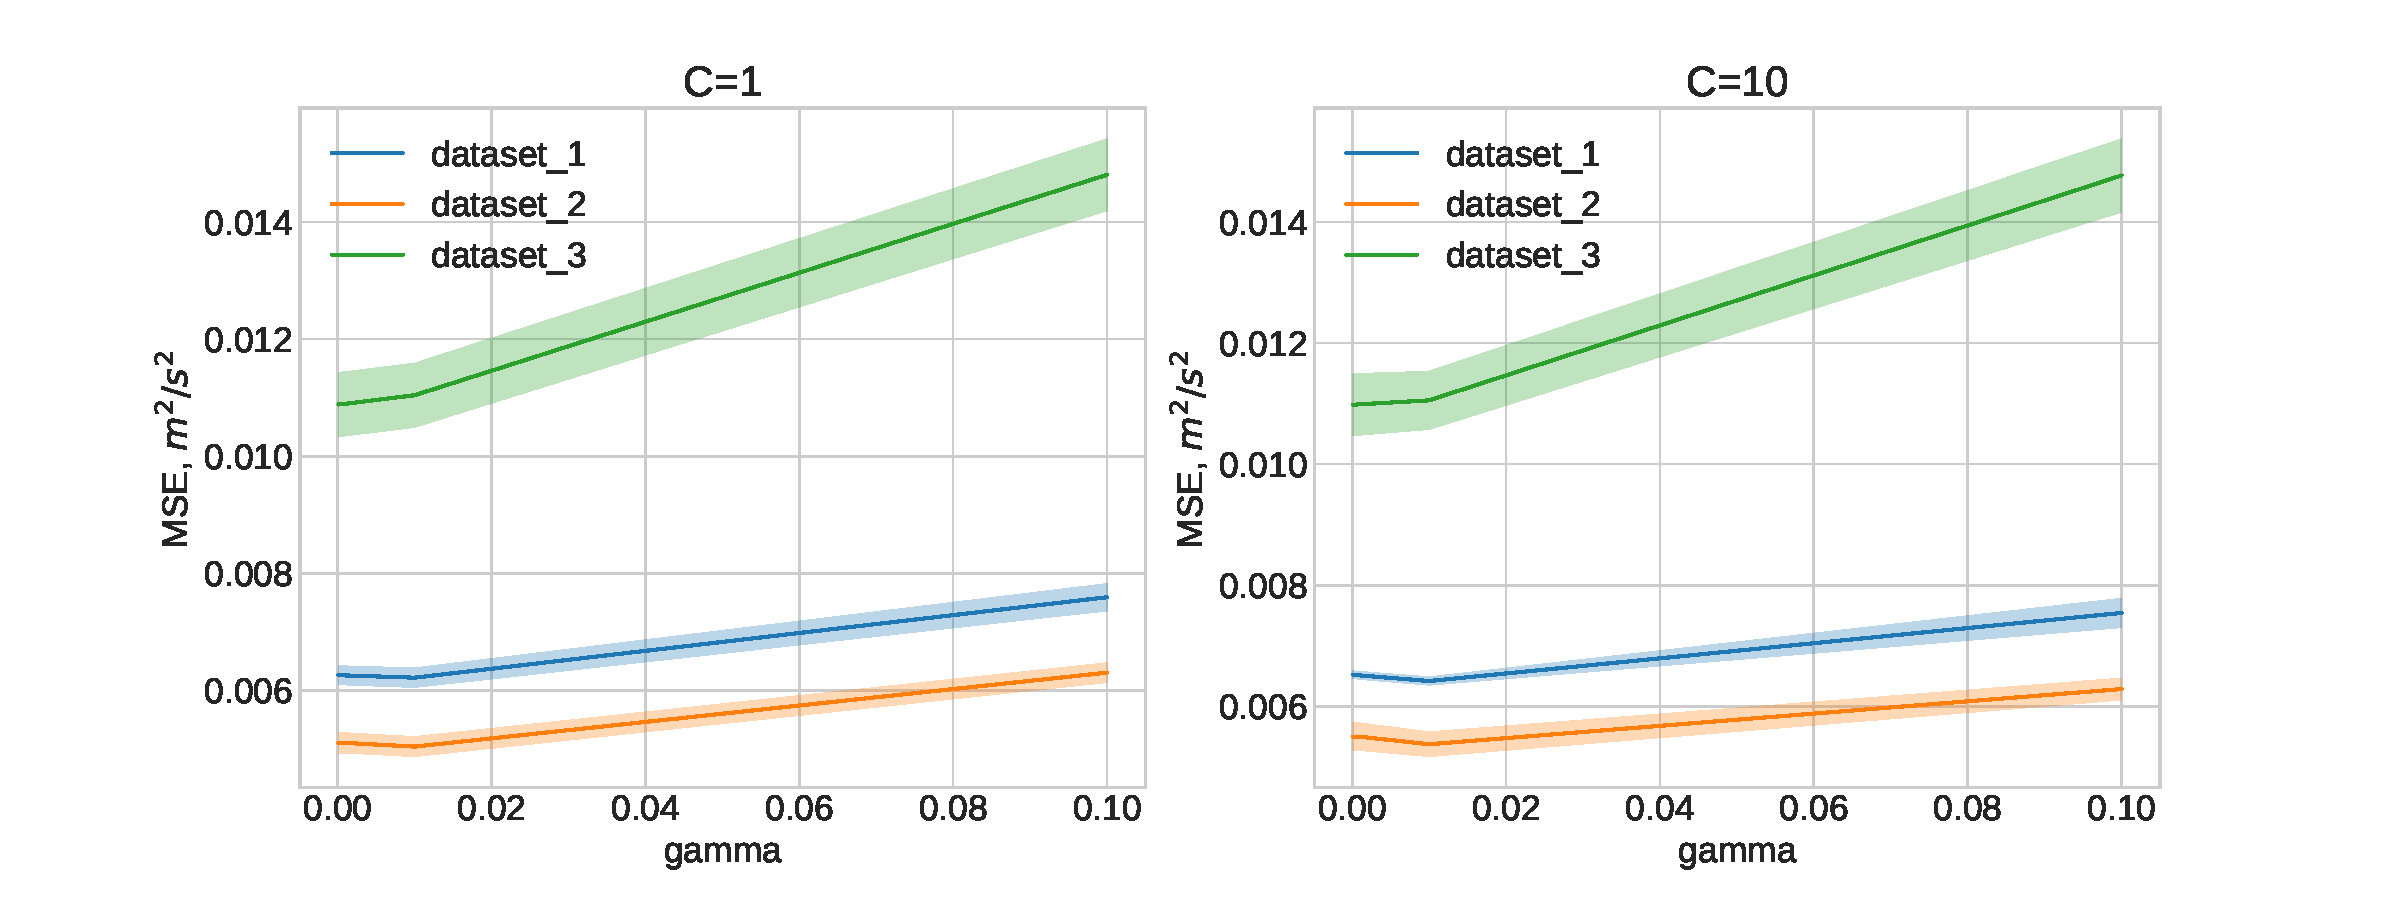
\includegraphics[scale=0.4]{charts/body_chn1_C=10.pdf}
    \caption{Тело, канал 1}
    \label{fig:image}
    \end{figure}
    

Для всех классов и выборок оптимальные значения параметра $\gamma$ близки к $0.001, 0.01$, поэтому при дальнейшем обучении моделей на большом количестве данных при заранее не заданных параметрах SVM-регрессоров, при поиске по сетке для параметра $\gamma$ будут использоваться только эти значения. Тогда для построенных моделей оптимальными параметрами будут следующие:

\begin{table}[H]
\begin{center}
\begin{tabular}{|c|c|c|c|c|}
\hline
& Рука & Нога & Сумка & Тело \\
\hline
C & 10 & 1 & 1 & 1 \\
\hline
$\gamma$ & 0.01 & 0.001 & 0.01 & 0.001\\
\hline
\end{tabular}
\end{center}
\end{table} 
    

По полученным значениям ошибок на кросс-валидации были выбраны оптимальные модели. С помощью этих моделей были построены траектории для каждого класса расположения смартфона (в качестве тестовой выборки была использована выборка Zhicheng). При этом траектории были построены для случаев, когда дополнительная корректировка весов с помощью оптимизации $V_{bias}$ не производилась (сиреневая линия) и когда производилась (синяя линяя). Истинная траектория обозначена красным цветом.


\begin{figure}[h]
\begin{minipage}[h]{0.49\linewidth}
\center{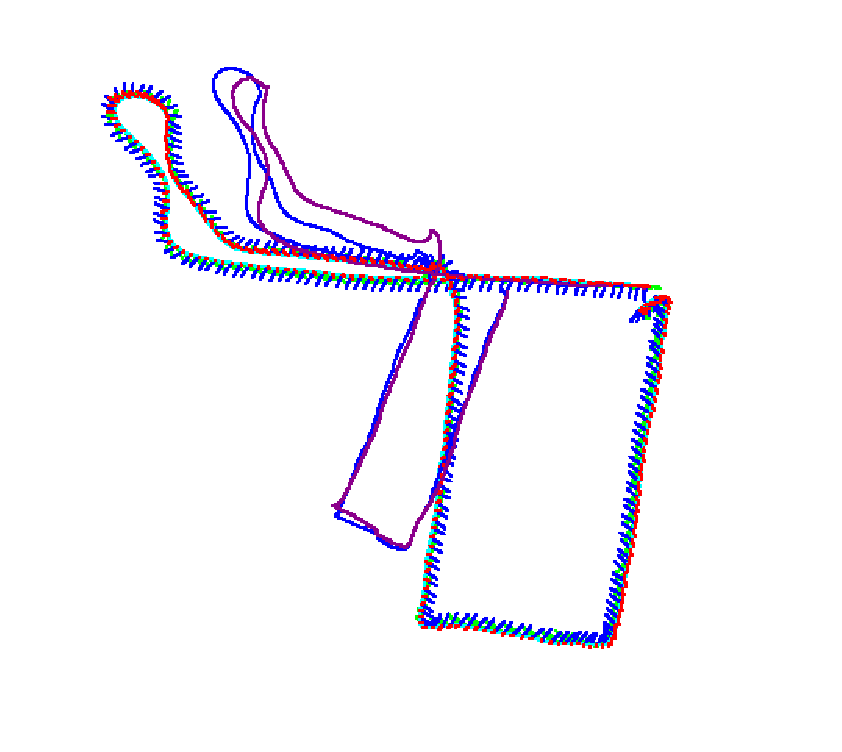
\includegraphics[width=0.5\linewidth]{trajectories/zhicheng_bag00.eps} \\ Класс-сумка}
\end{minipage}
\hfill
\begin{minipage}[h]{0.49\linewidth}
\center{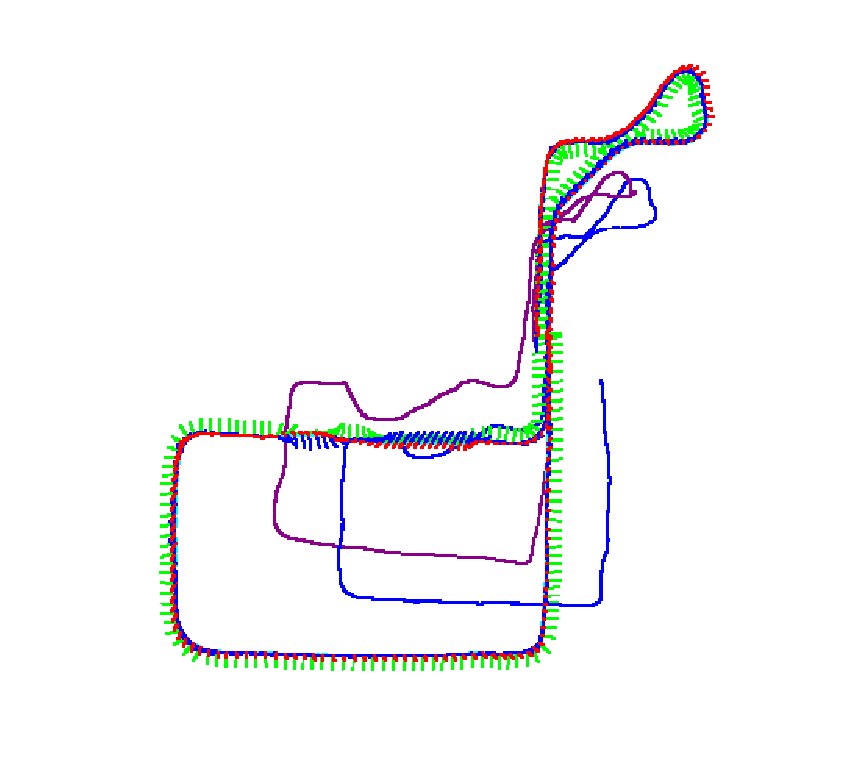
\includegraphics[width=0.5\linewidth]{trajectories/zhicheng_handheld00.eps} \\ Класс-рука}
\end{minipage}
\caption{Траектории}
\label{ris:image1}
\end{figure}

\begin{figure}[h]
\begin{minipage}[h]{0.49\linewidth}
\center{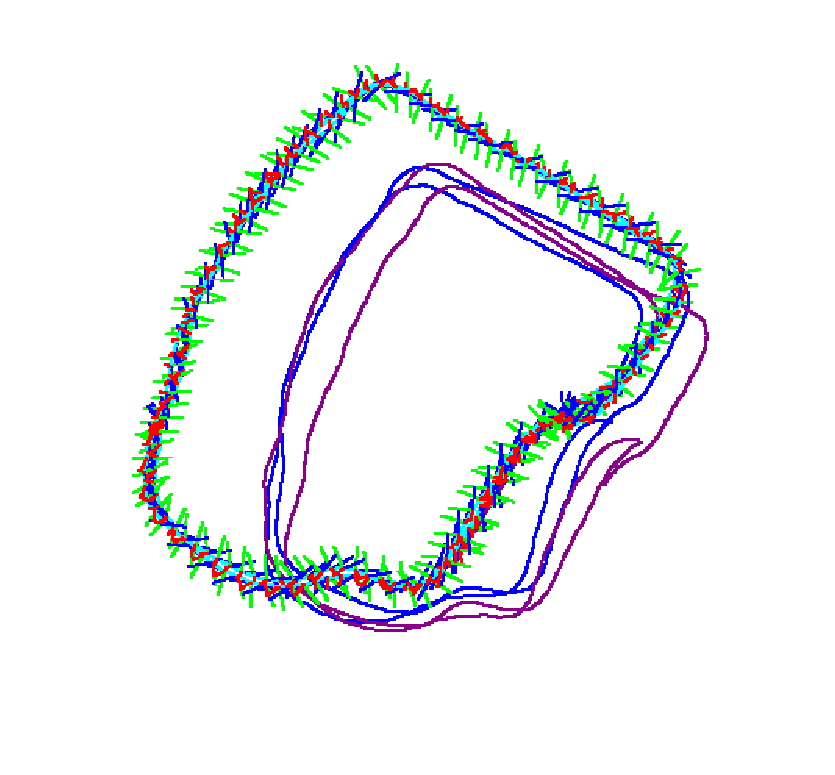
\includegraphics[width=0.5\linewidth]{trajectories/zhicheng_leg00.eps} \\ Класс-нога}
\end{minipage}
\hfill
\begin{minipage}[h]{0.49\linewidth}
\center{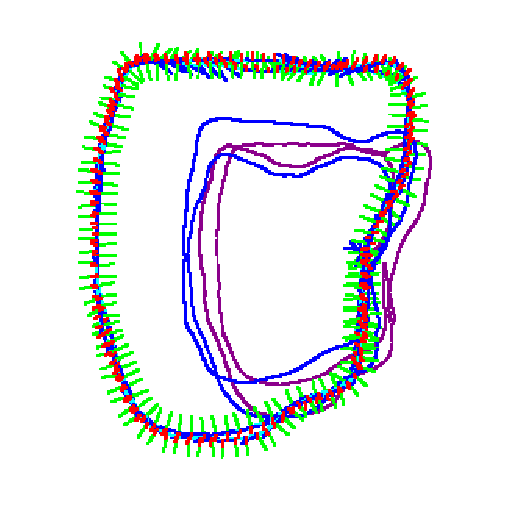
\includegraphics[width=0.5\linewidth]{trajectories/zhichenng_body00.eps} \\ Класс-тело}
\end{minipage}
\caption{Траектории}
\label{ris:image1}
\end{figure}

\section{Выводы}

Путем изначального определения расположения смартфона у человека(класс в данной задаче), были подобраны более подходящие параметры для моделей, которые увеличили точность построенных траекторий.

В ходе данной работы были повторены результа статьи для алгоритма RIDI~\cite{journals/corr/abs-1712-09004}. При работе с данными и для их улучшения был использован фильтр Гаусса.

В дальнейшем планируется применить полученную модель для дополнительно собранных данных, а также улучшить методы обработки данных для уменьшения шума (применение фильтра Калмана) и посмотреть другие способы оптимизации модели.



\newpage
\section{Приложения}
\rotatebox{90}{ %это обеспечивает поворот любого объекта
\begin{minipage}{1.5\linewidth}
\begin{table}[H]
\caption{Зависимости MSE ($m^2/s^2$) от параметров моделей для выборки 1}
\begin{center}
\begin{tabular}{|c|c|c|c|c|c|c|c|c|}
\hline
& \multicolumn{4}{c|}{C=1} & \multicolumn{4}{c|}{C=10} \\
\cline{2-9}
\raisebox{1.5ex}[0cm][0cm]{Регрессор}
& $\gamma=0.0001$ & $\gamma=0.001$ & $\gamma=0.01$ & $\gamma=0.1$
& $\gamma=0.0001$ & $\gamma=0.001$ & $\gamma=0.01$ & $\gamma=0.1$ \\
\hline
Сумка, 0
& $0.00949$ & $0.00948$ & $0.00944$ & $0.01025$
& $0.01032$
& $0.01029$
& $0.01011$
& $0.01051$ \\
\hline
Сумка, 1
& $0.00676$
& $0.00676$
& $0.00671$
& $0.00809$
& $0.00716$
& $0.00714$
& $0.00703$
& $0.00826$ \\
\hline
Тело, 0
& $0.00205$
& $0.00205$
& $0.00206$
& $0.00448$
& $0.00213$
& $0.00212$
& $0.00212$
& $0.00448$ \\
\hline
Тело, 1
& $0.00626$
& $0.00626$
& $0.00622$
& $0.00759$
& $0.00652$
& $0.00651$
& $0.00642$
& $0.00754$ \\
\hline
Рука, 0
& $0.00614$
& $0.00613$
& $0.00604$
& $0.00683$
& $0.00734$
& $0.00731$
& $0.00702$
& $0.00689$ \\
\hline
Рука, 1
& $0.01494$
& $0.01492$
& $0.01479$
& $0.0152$
& $0.01512$
& $0.0151$
& $0.01496$
& $0.01568$ \\
\hline
Нога, 0
& $0.00463$
& $0.00464$
& $0.00473$
& $0.00751$
& $0.00456$
& $0.00457$
& $0.00469$
& $0.00751$ \\
\hline
Нога, 1
& $0.00898$
& $0.00898$
& $0.00905$
& $0.01142$
& $0.00862$
& $0.00863$
& $0.00873$
& $0.01131$ \\
\hline

\end{tabular}
\end{center}
\end{table} 

\begin{table}[H]
\caption{Зависимости MSE ($m^2/s^2$) от параметров моделей для выборки 2}
\begin{center}
\begin{tabular}{|c|c|c|c|c|c|c|c|c|}
\hline
& \multicolumn{4}{c|}{C=1} & \multicolumn{4}{c|}{C=10} \\
\cline{2-9}
\raisebox{1.5ex}[0cm][0cm]{Регрессор}
& $\gamma=0.0001$ & $\gamma=0.001$ & $\gamma=0.01$ & $\gamma=0.1$
& $\gamma=0.0001$ & $\gamma=0.001$ & $\gamma=0.01$ & $\gamma=0.1$ \\
\hline
Сумка, 0
& $0.0125$
& $0.0125$
& $0.01255$
& $0.01519$
& $0.01232$
& $0.01232$
& $0.01234$
& $0.01521$\\
\hline
Сумка, 1
& $0.01013$
& $0.01013$
& $0.01029$
& $0.01406$
& $0.01051$
& $0.01051$
& $0.01065$
& $0.01406$ \\
\hline
Тело, 0
& $0.00205$
& $0.00205$
& $0.00206$
& $0.00448$
& $0.00213$
& $0.00212$
& $0.00212$
& $0.00448$ \\
\hline
Тело, 1
& $0.00511$
& $0.00511$
& $0.00504$
& $0.00631$
& $0.0055$
& $0.0055$
& $0.00537$
& $0.00629$ \\
\hline
Рука, 0
& $0.02699$
& $0.02699$
& $0.02676$
& $0.02657$
& $0.02176$
& $0.02176$
& $0.02155$
& $0.02282$ \\
\hline
Рука, 1
& $0.0246$
& $0.0246$
& $0.02451$
& $0.02552$
& $0.02342$
& $0.02342$
& $0.0234$
& $0.02541$ \\
\hline
Нога, 0
& $0.0054$
& $0.0054$
& $0.00546$
& $0.00789$
& $0.00544$
& $0.00544$
& $0.0055$
& $0.00789$ \\
\hline
Нога, 1
& $0.01289$
& $0.01289$
& $0.01295$
& $0.01489$
& $0.0131$
& $0.0131$
& $0.01306$
& $0.01488$ \\
\hline

\end{tabular}
\end{center}
\end{table} 
\end{minipage}
} 

\rotatebox{90}{ %это обеспечивает поворот любого объекта
\begin{minipage}{1.5\linewidth}
\begin{table}[H]
\caption{Зависимости MSE ($m^2/s^2$) от параметров моделей для выборки 3}
\begin{center}
\begin{tabular}{|c|c|c|c|c|c|c|c|c|}
\hline
& \multicolumn{4}{c|}{C=1} & \multicolumn{4}{c|}{C=10} \\
\cline{2-9}
\raisebox{1.5ex}[0cm][0cm]{Регрессор}
& $\gamma=0.0001$ & $\gamma=0.001$ & $\gamma=0.01$ & $\gamma=0.1$
& $\gamma=0.0001$ & $\gamma=0.001$ & $\gamma=0.01$ & $\gamma=0.1$ \\
\hline
Сумка, 0
& $0.00579$
& $0.00579$
& $0.00573$
& $0.00748$
& $0.00592$
& $0.00591$
& $0.00583$
& $0.00753$ \\
\hline
Сумка, 1
& $0.00242$
& $0.00241$
& $0.00239$
& $0.0041$
& $0.00247$
& $0.00247$
& $0.00241$
& $0.00435$ \\
\hline
Тело, 0
& $0.00379$
& $0.00379$
& $0.00389$
& $0.0065$
& $0.00384$
& $0.00384$
& $0.00391$
& $0.0065$ \\
\hline
Тело, 1
& $0.00511$
& $0.00511$
& $0.00504$
& $0.00631$
& $0.0055$
& $0.0055$
& $0.00537$
& $0.00629$ \\
\hline
Рука, 0
& $0.02699$
& $0.02699$
& $0.02676$
& $0.02657$
& $0.02176$
& $0.02176$
& $0.02155$
& $0.02282$ \\
\hline
Рука, 1
& $0.01025$
& $0.01024$
& $0.01016$
& $0.01158$
& $0.00991$
& $0.00989$
& $0.00975$
& $0.01072$ \\
\hline
Нога, 0
& $0.00394$
& $0.00395$
& $0.00401$
& $0.00614$
& $0.00403$
& $0.00403$
& $0.00405$
& $0.00609$ \\
\hline
Нога, 1
& $0.00649$
& $0.0065$
& $0.00659$
& $0.009$
& $0.00666$
& $0.00665$
& $0.00669$
& $0.00899$ \\
\hline

\end{tabular}
\end{center}
\end{table} 
\end{minipage}}





\bibliographystyle{plain}
\bibliography{literature}


\end{document}
